\chapter{Theoretische Grundlagen}
\label{chap:theoretical-basics}

\section{Das Rubidium-Atom}

\noindent Als Alkalimetall befindet sich Rubidium  in der ersten Hauptgruppe des Periodensystems und besitzt gemäß dem Bohr'schen Atommodell vier gefüllte Schalen und ein Valenzelektron in seiner äußersten Schale. Dadurch wird es als wasserstoffähnlich angenommen und es ergibt sich folgende Elektronenkonfiguration: $[\text{Kr}]5s^{1}$\\
\noindent Im Allgemeinen liegt der Anteil des natürlich vorkommenden $^{85}\text{Rb}$ bei $\approx72\%$ und der des $^{87}\text{Rb}$ bei $\approx28\%$ (\cite[S. ]{H2}). Beide Isotope unterscheiden sich sowohl in ihrer Masse (\cite{MassRb}), als auch in ihrem Kernspin \cite{H2}.

\begin{align}
    m_{85} & \approx \SI{84,9118}{u}, && I_{85} = 5/2 \\
    m_{87} & \approx \SI{86,9092}{u}, && I_{87} = 3/2 
\end{align}

\noindent Die Schmelztemperatur von Rubidium befindet sich bei $T_{\text{M}} = \SI{39,3}{\celsius}$ und seine Siedetemperatur bei $T_{\text{B}} = \SI{688}{\celsius}$ (\cite{Steck85} Table 2). Ebenso nehmen wir für das folgende Experiment an, dass beide Isotope stabil sind, obwohl $^{87}\text{Rb}$ als radioaktiver $\beta$-Strahler in $^{87}\text{Sr}$ mit einer zur Messzeit verhältnismäßig großen Halbwertszeit von ${t_{1/2}}= 4,7 \cdot 10^{10}a$ zerfällt. \cite{HWZ}\\

\noindent Im Folgenden soll nun allgemein auf die Aufspaltung der Energieniveaus wasserstoffähnlicher Atome eingegangen und sämtliche Korrekturen bis hin zur Hyperfeinstruktur erläutert werden.

\subsection{Grobstruktur}

\noindent Die mathematische Herleitung der quantisierten Energieniveaus ${E_{n}}$ eines wasserstoffähnlichen Systems folgt aus der nicht relativistischen, zeitunabhängigen Schrödingergleichung unter Verwendung des Coulombpotentials. Dabei bilden die Wellenfunktionen $\Psi_{n,\ell,m}$ einen Satz an Eigenfunktion des Hamiltonoperators $\hat{H}$ und erfüllen folgende Eigenwertgleichung.

\begin{align}
    \hat{H}\ket{\Psi_{n,\ell,m}}= E_{n}\ket{\Psi_{n,\ell,m}}
\end{align}

\noindent Die Eigenernergien ${E_{n}}$ ergeben die quantisierte Lage der Energieniveaus und werden allein durch die Hauptquantenzahl $n$ bestimmt:
\begin{align}
    E_{n} = - \frac{1}{2}m_{e}(c\alpha)^2\frac{Z^2}{n^2} \label{eq:Energielevel}
\end{align}

\noindent Unter Berücksichtigung relativistischer Korrekturen wie der relativistischen Massenzunahme und dem Darwinterm werden die in \eqref{eq:Energielevel} erhaltenen Energieniveaus jeweils um den Faktor $\alpha^2 \approx 10^{-4}$ angepasst. \cite{DemE4}\\

\subsection{Feinstruktur}

\noindent Die Spin-Bahn-Kopplung ist maßgeblich für die Feinstrukturaufspaltung verantwortlich. Dabei erzeugt das auf einer Kreisbahn um den Atomkern kreisende Elektron als elektrischer Kreisstrom ein magnetisches Dipolmoment, welches proportional zum Bahndrehimpuls $\ell$ ist.

%\begin{align}
  %  \mu_{\ell}= - \frac{e}{2m_{e}} \cdot \ell
%\end{align}

\noindent Im Ruhesystem des Elektrons hingegen rotiert der Atomkern um das $e^{-}$, induziert einen Kreisstrom und erzeugt am Ort des Elektrons ein Magnetfeld in dem der Spin des $e^{-}$ entlang der Quantisierungsachse die Werte $s_{z} { = \pm \frac{1}{2}\hbar}$ annimmt. Durch die Wechselwirkung zwischen dem magnetischen Spinmoment $\bs{\mu_{s}}$ und dem Magnetfeld welches durch die Bahnbewegung des Elektrons erzeugt wird, resultiert die Wecheslwirkungsenergie $\Delta E_{\ell,s} = -\bs{\mu}_{s} \cdot \bs{B}$ die die Eigenenergien aus \eqref{eq:Energielevel} folgendermaßen aufspaltet:

\begin{align}
    E_{n,\ell,s} = E_{n}-\bs{\mu_{s}} \cdot \bs{B} = E_{n} + \frac{\mu_{0}Ze^2}{8\pi m_{e}^2r^{3}}\cdot (\hat{\bs{S}} \cdot \hat{\bs{L}}) = \hat{H}_{LS} \label{EnergieFS}
\end{align}

\noindent Die Drehimpulsquantenzahl $\ell$ die für jede Hauptquantenzahl $n$ ganzzahlige Werte für $\ell \leq n- 1 $ annimmt, definiert das Intervall $-\ell \leq m \leq + \ell$ der für die magnetische Quantenzahl m möglichen Werte. Diese wird als Projektion des Drehimpulsoperators auf die Quantisierungsachse aufgefasst und ist äquivalent zu $\ell_{z}$. Daraus ergeben sich zu jedem $\ell$, $(2\ell +1)$ energetisch gleiche Unterzustände und die Eigenergien $E_{n}$ sind $n^2$-fach entartet. \cite{Bloch}\\

\noindent Für den Gesamtdrehimpuls und die zugehörige Eigenwertgleichung in der Feinstruktur unter Berücksichtigung des Elektornenspins gilt:
\begin{align}
    &\bs{j}=\bs{\ell} + \bs{s}\\
    &\bs{j}\ket{\Psi_{n, \ell, m}}=\sqrt{j(j+1)}\hbar\ket{\Psi_{n,\ell,m}}\label{eq:Eigenwerte}\\ 
    &j \in [\ell - s, \ell + s]
\end{align}
\noindent Analog zu \eqref{eq:Eigenwerte} können die Eigenwerte von $\bs{\ell}$ und $\bs{s}$ bestimmt werden.


\subsection{Hyperfeinstruktur}

\noindent Unter der Annahme der Atomkern sei räumlichen Ausgedehnt, wird auch diesem ein Spin -- der Kernspin $\bs{I}$ -- mit Eigenwerten $\bs{I}\ket{\Psi_{n, \ell, m}}=\sqrt{I(I+I)}\hbar\ket{\Psi_{n,\ell,m}}$ zugeschrieben. Das damit verknüpfte magnetische Kernmoment $\mu_{K}$ wechselwirkt mit dem Magnetfeld, welches durch die Bahnbewegung des Elektrons erzeugt wird und spalten  die Energieniveaus aus \eqref{EnergieFS} in Hyperfeinstrukturkomponenten auf.

%\begin{align}
   % &E_{\text{HFS}}= E_{n,\ell, j} + \frac{A}{2}[F(F+1)-j(j+1)-I(I+1)]\\
   % &A = \frac{g_{\ell}\cdot\mu_{K}\cdot B_{j}}{\sqrt{j(j+1)}} \label{eq:Hyperfeinkonstante}
%\end{align}

\noindent Aus der Kopplung des Gesamtbahndrehimpulses $\bs{j}$ mit dem Kernspin $\bs{I}$ folgt der Gesamtdrehimpuls des Atoms $\bs{F}=\bs{j}+\bs{I}$ mit Betrag $\lvert \bs{F} \rvert = \sqrt{F(F+1)}\hbar$. Dabei nimmt F$\in$ $[\lvert j-I\rvert;\lvert j+I\rvert]$ für jedes $j$ ganzzahlige Werte an.

\subsection{Auswahlregeln und Notation}

\noindent Um einen Atomzustand vollständig durch seine Quantenzahlen $(n,\ell,m)$ zu beschreiben, wird die spektroskopische Notation $n^{2s+1}L_{j}$ verwendet. Dabei wird L gemäß \ref{tab:Atomzustände} ersetzt.

\noindent Aufgrund folgender Auswahlregeln sind die Möglichkeiten eines Dipolübergangs limitiert:
\begin{multicols}{2}
\begin{itemize}
    \item $\Delta \ell = \ell_{1} - \ell_{2} \overset{!}{=} \pm 1$
    \item  $\Delta m_{\ell,1,2} = m_{\ell,1} - m_{\ell,2} \in \bigl\{-1,0, 1\bigr\}$ \\
    \item $\Delta j = j_{1} - j_{2} \in \bigl\{-1, 0, 1\bigr\}$ es sei denn, $j_{1} = j_{2} = 0$
    \item Interkombinationsverbot: Erhaltung der Multiplizität $2S+1$ bei Dipolübergang
\end{itemize}
\end{multicols}

\begin{table}[h]
    \centering
    \begin{tabular}{c|cccc}
         L &S &P &D &F \\
         \hline
         $\ell$ &0 &1 &2 &3\\
    \end{tabular}
    \caption{Zustände L gemäß der Drehimpulsquantenzahlen $\ell$}
    \label{tab:Atomzustände}
\end{table}

\noindent Für die Auswertung der $D_{2}$ Linie des Rubidium Atoms betrachten wir die Hyperfeinstrukturaufspaltung des Übergangs $5^{2}S_{1/2} \leftrightarrow 5^{2}P_{3/2}$ für den Grundzustand $n=5$ beider Isotope. Gemäß der in diesem Kapitel erarbeiteten Auswahlregeln, der spektroskopischen Notation sowie der Definition des Gesamtdrehimpulses F resultiert für $^{85}\text{Rb}$ und $^{87}\text{Rb}$ eine Aufspaltung der Energieniveaus wie in Abbildung \ref{fig:termschema} dargestellt. Aufgrund der Massendifferenz ergibt sich, wie in Abbildung \ref{fig:isotopieverschiebung} erkennbar, eine Verschiebung der Energieniveaus, was im Allgemeinen als \textbf{Isotopieverschiebung} bezeichnet wird. 

\begin{figure}[!h]
    \centering
    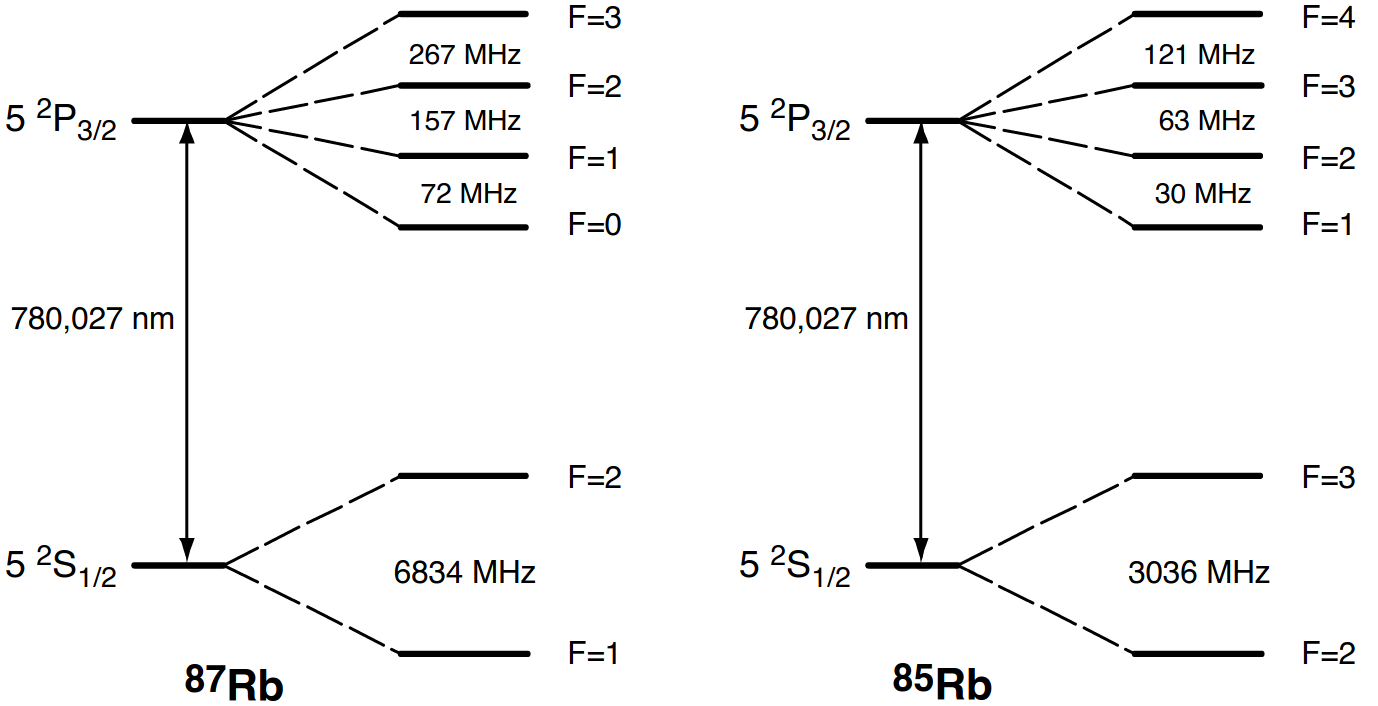
\includegraphics[scale = 0.45]{figures/images/termschema.png}
    \caption{Termschema für die Isotope $^{85}$Rb und $^{87}$Rb [Quelle: \cite{Krükow}, S. 5]}
    \label{fig:termschema}
\end{figure}

\begin{figure}
    \centering
    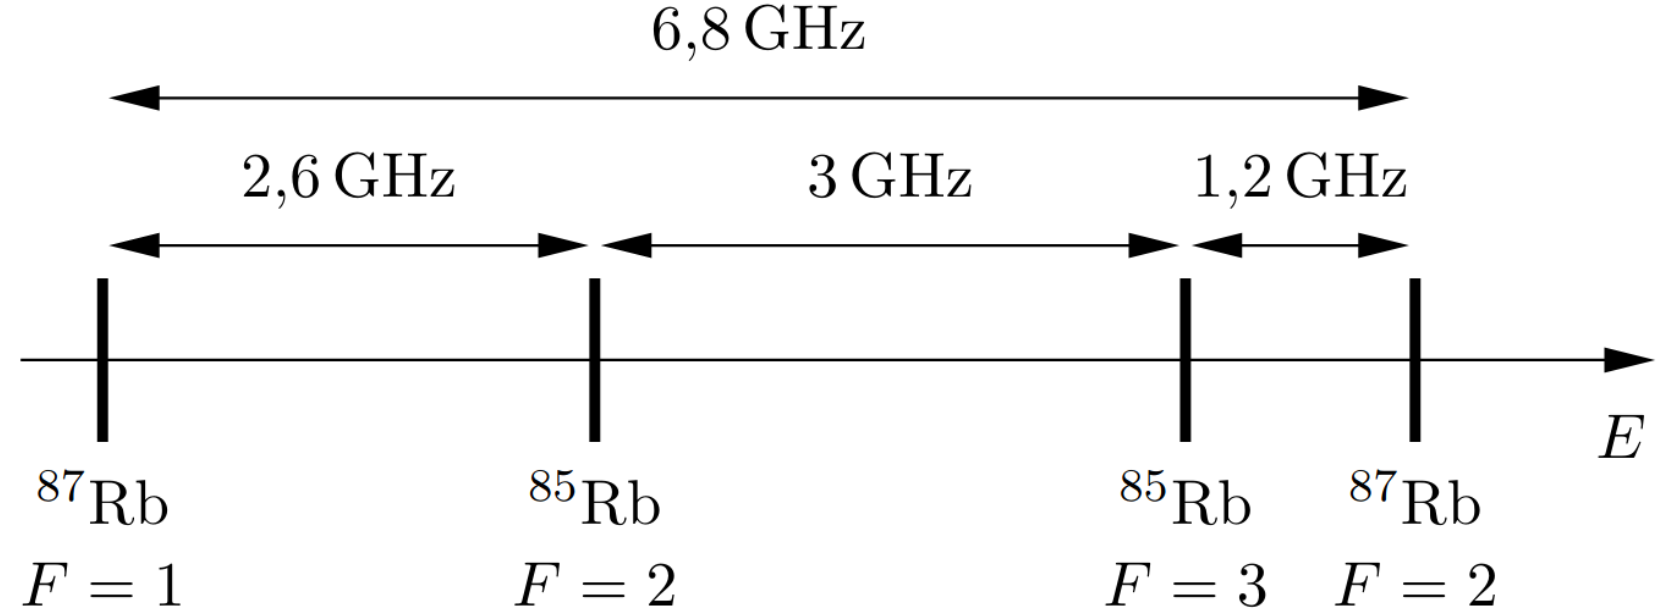
\includegraphics[scale = 0.28]{figures/images/isotopieverschiebung.png}
    \caption{Isotopieverschiebung [Quelle: \cite{Krükow}, S. 5]}
    \label{fig:isotopieverschiebung}
\end{figure}

\section{Laserspektrosopie}


 \noindent Um anhand der zwei gängigsten laserspektroskopischen Methoden -- die am Ende dieses Kapitels genauer betrachtet werden -- das Experiment durchführen zu können, ist die kontinuierliche Durchstimmung der emittierten Frequenzen der AlGaAs Laser Diode essenziell. Grund dafür ist, dass die Emission eine Laserdiode durch Bandübergänge innerhalb des Halbleiters hervorgerufen wird und nicht wie bsp.--weise im HeNe-Laser durch Elektronenstöße und atomare Übergänge die im Absorptionsspektrum scharf gepeakt sind. Der resultierende breite Verstärkungsbereich ($\approx \SI{100}{\nano \meter}$) ist größer als der freie Spektralbereich des internen Resonators der Diode, wodurch ein Mehrmoden-Betrieb ermöglicht wird. Der hier verwendete Halbleiterlaser basiert auf der Anwendung von Heterostrukturen in einem ternären Mischsystem. Im Allgemeinen ist über die Legierung des Al$_{x}$Ga$_{1-x}$As Halbleiters die Bandlücke und daraus resultierend die Energie $E_{G}$ für den Heteroübergang, der dem gleichen Funktionsprinzip wie der klassische p-n Übergang folgt, variabel und für den Verwendungszweck anpassbar. \cite{Hunkl}\\

\begin{figure}[!h]
    \centering
    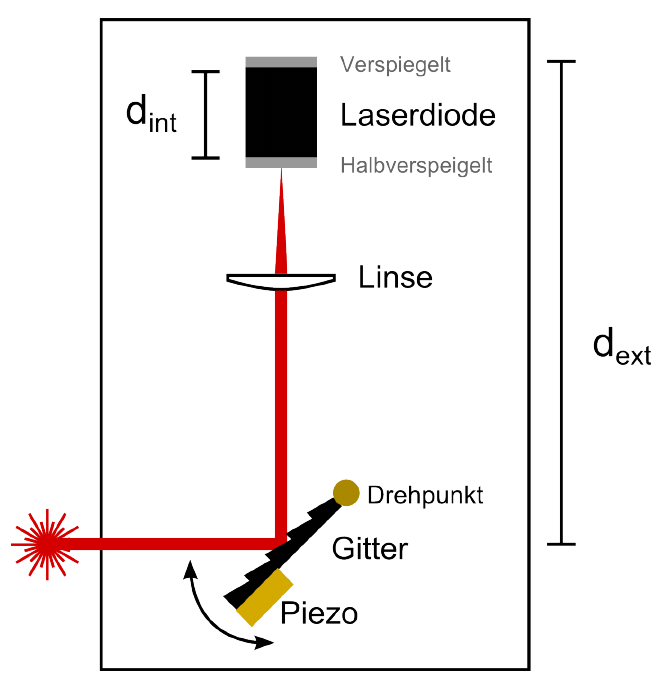
\includegraphics[scale = 0.4]{figures/images/diodenlaser.png}
    \caption{Aufbau eines Diodenlasers [Quelle: \cite{H2}, S. 21]}
    \label{fig:littrowgitter}
\end{figure}

\noindent Unter Verwendung eines drehbaren \textbf{Littrow-Gitters}, welches durch die Ausdehnung eines an Spannung angeschlossenen Piezo-Elements in Bewegung gesetzt wird, entsteht ein frequenzselektiver externer Resonator, der das 1. Beugungsmaximum am Gitter in die Laserdiode zurückreflektiert. Diese Konfiguration, abgebildet in \ref{fig:littrowgitter}, führt zu einem Einmoden-Betrieb, wenn ein deutliches globales Maximum im kombinierten Verstärkungsprofil existiert. Für die Gesamtverstärkung betrachtet man neben der Verstärkung des Lasermediums und der frequenzabhängigen Reflektivität des Gitters auch die Transmission sowohl vom internen Resonator der Diode $T_{int}$ als auch vom externen Resonator $T_{ext}$. Die emittierte Frequenz des Laser entspricht dabei, der Frequenz bei maximaler Verstärkung. Durch die Drehung des Gitters ändert sich der Gitterwinkel und die Länge des externen Resonators, wobei anhand der Wahl des Drehpunktes die reflektierten Resonanzen und die Verstärkung des externen Resonators synchron verschoben werden können, um im kombinierten Verstärkungsprofil ein Maximum beizubehalten. Um Modensprünge in der Gesamtverstärkung zu vermeiden, wird der Strom im Halbleiterlaser erhöht, was neben dem Brechungsindex n auch die optische Weglänge im internen Resonator erhöht. \cite{H2}\\

 \noindent Im folgenden werden Begriffe, Apperaturen und Methoden die für die spektroskopische Untersuchung am Rubidium essenziell waren, erklärt.

\subsection{Linienbreite}

\noindent Die absorbierte und emittierte Strahlung eines atomaren Übergangs in einem 2-Niveau-System ist nicht streng monochromatisch, sondern weist Frequenzen nahe der Resonanzbedingung (\ref{eq:Resonanzbedingung}) auf, wodurch die Übergangsenergien nicht beliebig scharf sind und die Spektrallinien eine \textbf{Linienbreite} besitzen.

\begin{align}
    \nu_{12}=(E_{2}-E_{1})/ h \label{eq:Resonanzbedingung}
\end{align}

\noindent Aus der Betrachtung der Energie-Zeit-Unschärfe, unter Berücksichtigung der endlichen aber auch mit einer Unschärfe behafteten Lebensdauer eines angeregten Energieniveaus $\tau$, resultiert eine endliche Energiebreite $\delta E= \frac{\hbar}{\delta \tau}$ die zu einer Frequenzbreite im Spektrallinienbild führt. Wodurch \ref{eq:Resonanzbedingung} zu \ref{eq:Frequenzbreite} wird.

\begin{align}
    \delta \nu_{12}=(\delta E_{2}-\delta E_{1})/ h \label{eq:Frequenzbreite}
\end{align}

\noindent Das Resultat wird im Allgemeinen als \textbf{natürliche Linienbreite} bezeichnet und lässt sich nicht durch Optimierung der Messapperatur eliminieren, da sie aus der quantenmechanischen Betrachtung folgt. Die Intensitätsverteilung einer Spektrallinie unter Einfluss der natürlichen Linienbreite ist lorentzförmig \ref{eq:natürliche Linienbreite}.

\begin{align}
    I(\omega)=I_{0}\frac{1}{\pi}\frac{\frac{\gamma}{2}}{(\omega-\omega_{0})^2+(\frac{\gamma}{2})^2} \label{eq:natürliche Linienbreite}
\end{align}

\noindent Eine weitere wichtige Form der Linienbreite, die für unserere spektroskopische Untersuchung eine zentrale Rolle spielt, ist die \textbf{Doppler-Verbreiterung}. Anschaulich gesprochen resultiert sie aus dem Bild, dass statistisch und aus Sicht des Laborystems alle Atome und Moleküle aufgrund ihrer thermischen Energie in Bewegung sind. Durch diese intrinsiche Bewegung verschiebt sich die Resonanzfrequenz eines Übergangs in Bezug zum Beobachter, woraufhin eine Linienverbreiterung zustande kommt.

\noindent Da die Wahrscheinlichkeit ein Atom bei einer bestimmten kinetischen Energie $E_{\text{kin}}$ vorzufinden gemäß Boltzmannstatistik proportional zu $\propto \exp(-\frac{E_{\text{kin}}}{k_{B}T})$ ist, folgt für die Wahrscheinlichkeitsverteilung der Geschwindigkeit entlang jeder Raumrichtung $i \in \{x,y,z\}$ einer Gauß-Verteilung:\\

\begin{align}
    p_{i}(v_{i}) = \sqrt{\frac{m}{2\pi k_{B}T}} \cdot \E^{- \frac{mv_{i}^2}{2k_{B}T}} \label{eq:Gaußverteilte Geschwindigkeit}\\\nonumber
\end{align}

\noindent Daraus ergibt sich für die Intensitätsverteilung $I(\omega)$ der Spektrallinien -- unter Einfluss der Dopplerverbreiterung -- ein gaußförmiger Verlauf. \cite{H2}

\begin{align}
    I(\omega) &= I(\omega_{0}) \cdot \exp \biggl[- \biggl(\frac{\omega-\omega_{0}}{\frac{\Delta \omega}{2\sqrt{\ln{2}}}}\biggr)^2 \biggr] \label{eq:gauss-intensity} \\
    \Delta \omega &= 2\sqrt{\ln 2} \frac{\omega_{0}}{c}\sqrt{\frac{2k_{B}T}{m}} \label{eq:delta-omega}
\end{align}
\newpage
\subsection{Optische Resonatoren}

\noindent Im Allgemeinen besteht ein \textbf{Fabry-Pérot-Resonator (FPI)} aus zwei zueinander parallelen Spiegeln, die einen einfallenden Laserstrahl zwischen sich hin und her reflektieren lassen und dabei an beiden Enden einen geringen Anteil absorbieren und transmittieren. Der reflektierte Strahl sammelt pro Umlauf eine Phase $\phi=2dk$ auf, wobei $d$ für den Spiegelabstand und $k$ für die Wellenzahl $k=\frac{2\pi}{\lambda}=\frac{\omega}{c}=2\pi\frac{\nu}{c}$ steht. Es kommt zu einer Interferenz zweier aufeinander folgender transmittierter Lichfelder, sobald die aufgesammelte Phase pro Umlauf einem ganzzahligen Vielfachen $n\in \N$ von $2\pi$ entspricht. In diesem Fall spricht man von einem sich reproduzierenden Strahl im Resonator.

\begin{align}
    \phi=2dk = 2d \frac{2\pi \nu_{n}}{c} \overset{!}{=} 2\pi \cdot n \label{eq:Interferenzbedingung}
\end{align}

\noindent Aus Gleichung \ref{eq:Interferenzbedingung} resultiert die Resonanzfrequenz $\nu_{n}$ des Resonators und damit folgt für den freien Spektralbereich $\nu_{\text{FSR}}$, der den Frequenzabstand zweier aufeinanderfolgender Resonanzen mit der Geometrie des Resonators kombiniert: 

\begin{align}
    \nu_{n}-\nu_{n-1}=\nu_{\text{FSR}}=\frac{c}{2d}
\end{align}

%\noindent Die Linienbreite $\Delta\nu = \frac{c}{2\pi d} (L+T)$ ist Abhängig von der Transmission T und der Absorbtion L beider Spiegel sowie von der Länge des Resonator. \cite{H2} Daraus folgt für die Finesse des Resonators $F=\frac{\nu_{FSR}}{\Delta\nu}=\frac{\pi}{L+T}$

\noindent Da der Laser aus unserem Experiment allerdings Gaußsche Strahlen generiert, die eine gekrümmte Wellenfront aufweisen, war es sinnvoll einen \textbf{konfokalen Resonator (KR)} zu verwenden, um sowohl die Einkopplung des Strahls in den Resonator zu gewährleisten, als auch dessen Reproduktion im Resonator sicher zu stellen. So können Verluste durch einen zunehmende Divergenz des Strahls minimiert werden. Im wesentlichen unterscheidet sich diese Anordnung durch seine gekrümmten Speigel vom zuvor diskutierten FPI. Auszeichnend für diese Art von Resonatoren ist, das der Krümmungsradius der Spiegel $R_{KR}$ der Resonatorlänge $d$ entspricht, wodurch sich der optische Weg im Vergleich zum FPI verdoppelt und damit der freie Spektralbereich halbiert -- für $d_{\text{FPI}}=d_{\text{KR}}$.

\begin{align}
    \nu_{\text{FSR}}=\frac{c}{4d} \label{eq:freier Spektral Bereich}
\end{align}

\subsection{Absorptions- \& Sättigungsspektroskopie}

\noindent Im Wesentlichen basieren beide spektroskopischen Methoden auf dem Prinzip, dass ein Laserstrahl durch eine Probe gesendet und im Anschluss die transmittierte Intensität in Abhängigkeit der Frequenz gemessen wird. Bei der \textbf{Absorptionsspektroskopie} zeichnet sich jeder atomare Übergang über einen Einbruch in der Intensität aus. Liegen allerdings zwei Übergänge im Bereich der Dopplerverbreiterung, die für Gase bei $T=\SI{300}{\kelvin}$ in etwa $\SI{1}{GHz}$ beträgt, erscheinen beide Übergänge im Transmissionsspektrum als eine verbreiterte Linie und können daher mittels dieser Methodik nicht aufgelöst werden. Im Falle des Rubidiums erwarten wir resultierend daraus gemäß Abbildung \ref{fig:termschema} pro Isotop zwei Peaks in unserem Spektrum. Durch die kontinuierliche Durchstimmung der Frequenzen wird das gesamte Spektrum abgedeckt. 

\noindent Anhand der \textbf{Sättigungsspektroskopie} können Übergänge, die zuvor im Absoropitonsspektrum nicht zu erkennen waren, dopplerfrei untersucht werden. Dafür lässt man zwei Teilstrahlen eines Laser -- Pump
- und Teststrahl -- in jeweils entgegengesetzter Richtung durch die Probe propagieren. Entspricht die Frequenz beider Strahlen der Übergangsfrequenz $\nu_{a}=\nu_{\text{Pump}}=\nu_{\text{Test}}$, sind alle Atome mit  $v_{z}=0$, die also keine Bewegung entlang der optischen Achse aufweisen, aufgrund der fehlenden Dopplerverschiebung mit beiden Teilstrahlen resonant. Da der deutlich stärkere Pumpstrahl den Übergang sättigt und ein Besetzungsgleichgewicht erzeugt, sinkt die Absorptionswahrscheinlichkeit des Teststrahls und dessen Transmission zeigt sich im Absorptionsspektrum als \textbf{Lamb-Peak}, wie in Abbildung  \ref{fig:lamb-peak} gezeigt. Alle weiteren Atome für die $v_{z}\neq 0$ gilt, sind nur mit einem der zu ihnen dopplerverschobenen Strahlen resonant, welche abhängig von der Bewegungsrichtung des Atoms in dessen Inertialsystem entweder rot- oder blauverschoben sind. Sobald der Teststrahl mit der Übergangsfrequenz resonant ist, befinden sich die Atome im Grundzustand, die Absorptionswahrscheinlichkeit des Teststrahls ist sehr hoch und es wird ein gaußförmiger Einbruch in der Transmission verzeichnet. 

\noindent Liegen im Falle der Sättigungsspektroskopie zwei Übergänge mit den Frequenzen $\nu_{a}$, $\nu_{b}$ im Bereich der Dopplerverbreiterung, macht sich dies im spektroskopischen Bild erkenntlich durch die in Abbildung \ref{fig:crossover-peak} auftretenden drei Peaks. Die zwei äußeren Lamb-Peaks resultieren wie zuvor schon aus den Atomen mit $v_{z}=0$ und der Resonanz beider Teilstrahlen mit jeweils einem Übergang. Zusätzlich wird allerdings die Laserfrequenz genau zwischen den zwei Übergangsfrequenzen auf $\nu_{L}=\frac{\nu_{a}+\nu_{b}}{2}$ gesetzt. Daraus folgt, dass es Atome mit den Geschwindigkeiten $\pm v_{c}$ gibt, bei denen aufgrund der gegenläufigen Dopplerverschiebung beide Teilstrahlen mit jeweils einer Übergangsfrequenz resonant sind. Während der Pumpstrahl den Übergang zu $\nu_{a}$ sättigt und somit ein Besetzungsgleichgewicht erzeugt, sinkt die Wahrscheinlichkeit für den Teststrahl die Atome in den Zustand zu $\nu_{b}$ anzuregen und dessen Transmission wird schließlich als \textbf{Cross-Over Peak}, mittig zwischen den beiden Lamb-Peaks auftretend, sichtbar. Da sowohl Atome mit $+v_{c}$ als auch Atome mit $-v_{c}$ zu einem Cross-Over Peak beitragen, ist dieser im spektroskopischen Bild wesentlich stärker zu erkennen als die Lamb-Peaks. Anhand der Breite der Geschwindigkeitsverteilung aus \ref{eq:Gaußverteilte Geschwindigkeit} und dem Abstand zwischen den beteiligten Übergängen lässt sich eine statistische Approximation für die Anzahl der zum Peak beitragenden Atome angeben. Für die Lamb-Peaks berechnet sich die Anzahl der beteiligten Atome über das Maximum von \ref{eq:Gaußverteilte Geschwindigkeit}.\cite{H2}


\begin{figure}[!h]
    \begin{minipage}{7cm}
        \centering
        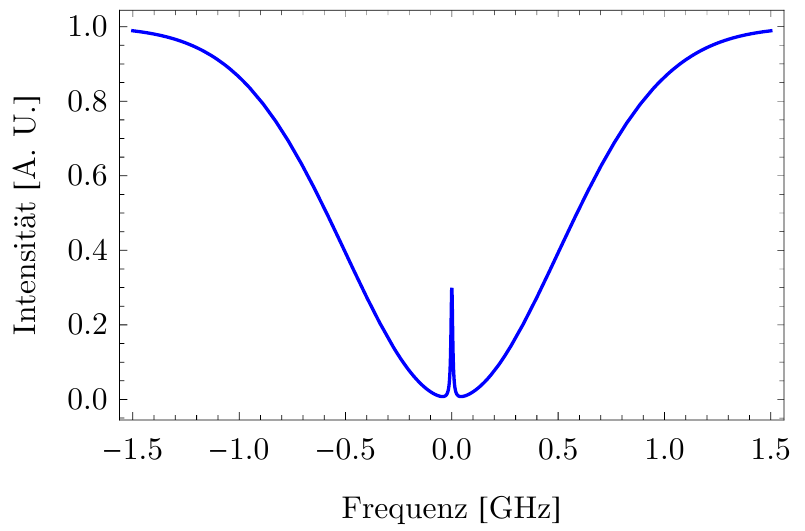
\includegraphics[scale = 0.4]{figures/images/lamb-peak.png}
        \caption{Lamb-Peak [Quelle: \cite{H2}, S. 26]}
        \label{fig:lamb-peak}
    \end{minipage}
    \hfill
    \begin{minipage}{8cm}
        \centering
        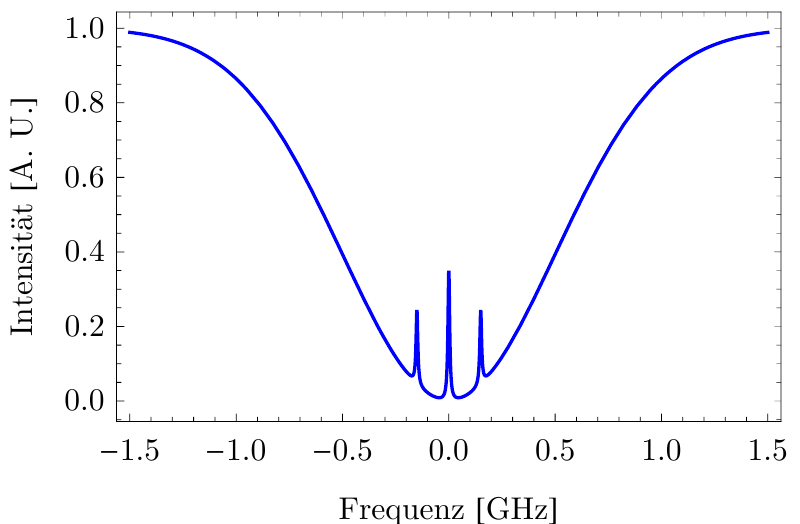
\includegraphics[scale = 0.4]{figures/images/cross-over-peak.png}
        \caption{Cross-Over Peak [Quelle: \cite{H2}, S. 30]}
        \label{fig:crossover-peak}
    \end{minipage}
\end{figure}


\cleardoublepage{}